\chapter{Introduction}
\subsection{Science with increasing resolution}

%Pr: 3. St : 2

%The structure of the introduction is to be altered considerably to be made shorter and clear. At the moment, I'm looking at basing the structure on Ben's Intro. This would entail moving the meat of the VLBI and EHT sections to the theoretical background 

%why go to high  resolution -> several examples (bh relations - HST, HL TAU-ALMA, bullet cluster - chandra??) of how an increase in resolution has lead to new physical insights. 

Throughout the history of astronomy, we see celestial sources which appear point-like or unresolved with the instrumentation available at the time. To study these sources in enough detail to clarify their nature, ever more sophiscated instruments have to be developed. 

These instruments span the electromagnetic spectrum, and here I recall several notable examples which illustrate the discovery potential of an increase in resolution.

At optical wavelengths, the Hubble Space Telescope was able to resolve the gravitational sphere of influence of the central supermassive black hole (SMBH) in nearby galaxies. These measurements uncovered the fundamental relations between black hole mass and both stellar bulge luminosities and velocity dispersions (Ferrasse and Merritt (2000), Gebhardt et al. (2000)) which has been a foundation for extra-galactic astronomy ever since. 

A more recent example is a 2014 science verification result with the Atacama Large Millimetre Array (ALMA) \cite{brogan_2015} which resolves the molecular dust disk surrounding the young protostellar system, HL Tau Fig.~\ref{fig:hl_tau}. This observation showed, in unique detail, the orbit cleared out by forming planets which was suprising given that the stellar system was so young. The clarity of the image surpasses all previous work on the subject and provides an strong science case for conducting observations of similiar systems with ALMA. 

\begin{figure*}
\begin{center}

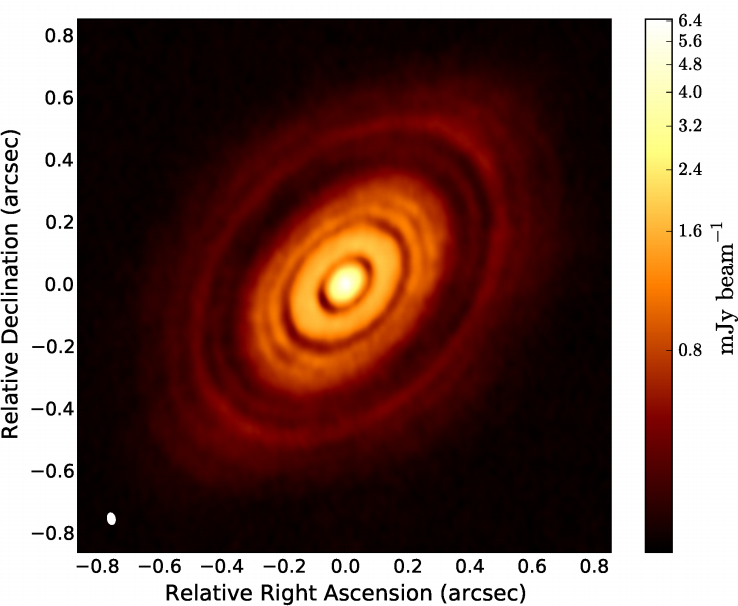
\includegraphics[width=\columnwidth]{Images/hl_tau}
\caption{The young stellar system HL Tau, observed at 223 GHz by ALMA. The orbits of forming planets appear as dark rings cut out of the disk. The presence of these bodies are suprising given that host star is still very young. The detail in this image was made possible by the milliarcsec resolution acheivable with ALMA. \label{fig:hl_tau}}

\end{center}
\end{figure*}

X-ray wavelengths with Chandra, we see the bullet cluster (Clowe 2004, )

The technique which acheives the highest resolution is Very Long Baseline Interferometry (VLBI)

\subsection{Very Long Baseline Interferometry}
%Pr : 3 St :3
% brief historical context of vlbi 

VLBI is  network 

The development of VLBI, originated in the late 1960's with observations of compact, highly-variable objects, now known as quasars. Teams using VLBI discovered that these objects consist of core-jet systems. Also the presence of super-luminal jet motion. \textit{TMS copy, paste : By using local
oscillators at each antenna that are controlled by high-precision frequency stan-
dards, it is possible to preserve the coherence of the signals for time intervals
long enough to measure interference fringes. The received signals are converted
to an intermediate frequency low enough that they can be recorded directly on
magnetic tape, and the tapes are subsequently brought together and played into
a correlator.}

% examples of arrays, with their specs

Examples of Arrays : Very Long Baseline Array (VLBA) : 1.4 - 87 GHz, European VLBI Network (EVN), African VLBI Network (AVN).  

\subsection{The Event Horizon Telescope (EHT)}
%Pr : 3, St: 3
This thesis is centred around such a class of emerging early 21st century instrumentation, known as Very Long Baseline Interferometry at millimetre wavelengths (mm-VLBI). This technique enables angular resolution on the order of $\sim 10\ \mu$-arcsec by maximising both antenna separation and observing frequency. The sub-field is being led by the Event Horizon Telescope consortium (EHT), an international project whose primary objective is to resolve the supermassive black holes  (SMBH) located at the centre on our Galaxy, known as Saggittarius~A$^\star$ (Sgr~A$^\star$), and M87 on angular scales comparable to the black hole event horizon. This thesis aims to contribute to the EHT objectives through algorthimic development of data simulation and parameter estimation pipelines, which are particularly relevant given the significant calibration challenges faced by the project.

\begin{figure*}
\begin{center}
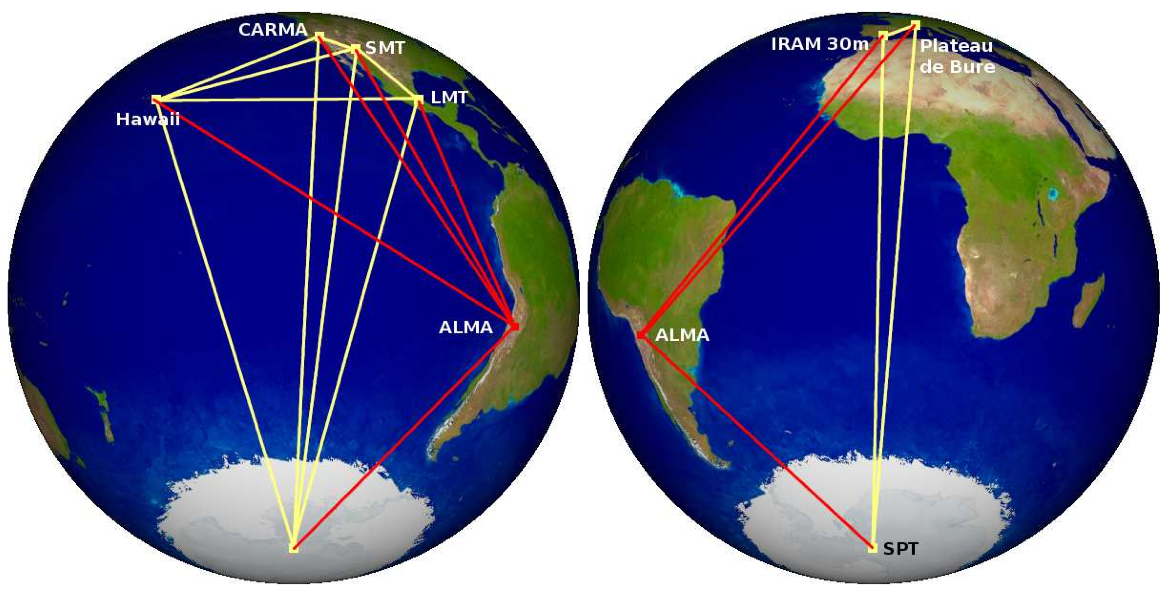
\includegraphics[width=\columnwidth]{Images/eht_globe}
\caption{(Image credit: Remo Tilanius) Event Horizon Telescope uses \textbf{Earth-diameter baselines} to attain \textbf{resolution} \boldmath$\sim 10$ $\mu$arcsec. \label{fig:eht_globe}%
}
\end{center}
\end{figure*}

\subsection{Scientific opportunities with the EHT}
%Pr : 3,  St:3
To constrain the physics near a black hole, the observation needs to be sensitive to scales comparable to the event horizon. For the case of a non-spinning or Schwarschild black hole, the event horizon is spherically symmetric with a radius, $R_{\rm Sch} = 2 G M_{\rm BH} /c^2$,  where $M_{\rm BH}$ is the black hole mass, $G$ is the gravitational constant and $c$ is the speed of light. The angular size of such an event horizon in the far field approximation is $\theta_{\rm Sch} = R_{\rm Sch} / D \approx 0.02$~nanoarcsec~($M_{\rm BH}/M_\odot$)(kpc/$D$) where $D$ is the distance from observer to source. For SMBH's Sgr~A$^\star$ and M87, this results in $\theta_{\rm Sch} \sim 5-10\ \mu$-arcsec. The event horizon telescope will have baseline lengths $|b| \sim 10^3$~km and is currently observing at $\nu =230$~GHz, yielding a diffraction-limited angular resolution of $\theta_{\rm EHT} = 1.22 \nu/ |b| \approx $. Hence EHT will be able to resolve these objects on the scale of the event horizon/gravitational radius. 

Equally important to  that the millimetre emission is optically thin and therefore probes inner emission region. The power spectrum of Sgr~A$^\star$ peaks in sub-mm bump. Synchtron emission. Lensed emission. the interferometric technique also filters out smooth mm emission.[Read Falke 1998]

{\bf FIG. basic grmhd image of black hole shadow, scale indicating resolution and eht beam size}\\


\subsubsection{Strong gravity and black hole spacetime}
%Pr : 3, St: 3
Gravity as described by General Relativity (GR) has flawlessly agreed with all observational experiments, however GR has conceptual weaknesses, especially as it is not compatible with the quantum description of reality. Various alternatives to GR have been theorised which do not assume a purely classical description of matter. To test GR against it's numerous alternatives, we have to observe gravity in the regime where we expect the largest observational deviations a GR prediction would have if it were only an approximate theory of gravity.  The spacetime close to a SMBH is an ideal candidate, as the gravitational effects are very strong. Lensed emission of the gravitational lensed photon ring.  The exact sizes and shapes of which indicate different spacetime and theories of gravity. Note that even in this regime, the deviation from GR is small. We can also explore black hole physics by testing the no-hair theorem or that black holes are only described by their mass, spin and charge by constraining the quadrapole moment of the black hole.deviations
from the Kerr metric

{\bf FIG. Plot of analytic shapes and sizes of the bh shadow from the predictions of different theories of gravity}\\
~\\
\subsubsection{AGN accretion and jet launch astrophysics} 

{\bf [AGN jet basics.]}

Astrophysical jets were first discovered over a century ago, accretion onto a black hole was first postulated to power these jet by .. .However a century later, the mechanism of accretion and jet launching ifrom SMBH are still highly debated. 

\textbf{Fig: Typical AGN jet illustration showing magnetic fields }

Recently an industry of sophiscated General Relativistic Magneto-Hydrodyanmic (GRMHD) simulations has developed yielding important insights but also new questions. Now, mm-VLBI has the opportunity of constrains the mechanisms. Specifically we can map the magnetic field configuration, which is a key aspect using polarimetry and Faraday Rotation. The quiescent and variability structure and also be explore in total intensity. Flaring structure.  Distiniguish between accretion disk and inner jet. Distinguish between the different Jet and Disk models for each bh. Deterimine spin.\\
~\\
\textbf{Fig: 2/3 panels of simulated images of disk and jet models of Sgr A*/M87}\\

In M87, where the jet is dominant, micro-arcsecond scale astrometry, capable with the EHT, can determine the distance from the jet base from the event horizon, as well as the width of the jet base. Opening up new possibilities in explore particle production and other exotic physics occuring at the event horizon. 


\textbf{Fig: 2/3 panels of simulated polarimetric images of Sgr A*/M87 showing ordered magnetic fields}
\subsection{Challenges and obstacles in mm-VLBI observations}
%Pr : 2, St : 2
%Overview of challenges
Performing Very Long Baseline Interometry (VLBI) at mm-wavelengths presents unique calibration challenges, including very short atmospheric coherence times that are typically $\lesssim$10~s \citep{Doeleman_2009}, low calibrator source sky density, complex and variable calibrator source structure, and antenna pointing accuracies that are a non-negligible fraction of the antenna primary beam. Addition These effects may place significant limitations on the sensitivity, image fidelity, and dynamic range that can be achieved with mm-VLBI.  Performing mm-VLBI however, is a difficult task for a variety of reasons. Firstly the arrays are inhomogenous, made up of a collections of different stations working together, Difficult to get time on all the stations. there are a variety of signal corruptions which take place. Briefly introduce signal corruptions, variability, ..etc, how these represent calibration and interpretation challenges.


\subsection{Science extraction : parameter estimation and imaging}
%Leave for now
%Pr : 2, St : 3

%High accuracy needed for science 
we need to measure the fractional
asymmetry of the shadow shape with respect to its angular size to the few percent

%Briefly discuss imaging, it's difficulties..\\

~\\
%parameter estimation through robust visibility derivatives
Estimating the `macro'-parameters of Sgr A*, spin, orientation, position angle through a Bayesian parameter estimation analysis with closure quantities\\
Furthermore, unaccounted for systematic and/or non-Gaussian uncertainties could preclude robust, accurate Bayesian parameter estimation and model selection analyses of accretion flow \citep[e.g.][]{Broderick_2016} and gravitational physics \citep[e.g.][]{Broderick_2014, Psaltis_2016}, two of the EHT's many objectives.
~\\
see psaltis 2015 for  some other shadow detection criteria
\textbf{Fig: A Broderick 2016 posterior probability distribution (?)}

\subsection{A realistic mm-VLBI simulator}
%Pr : 1 : St : 1

%Why simulate: intro
Given the significant observation challenges that the EHT faces, we have undertaken this project to build a mm-VLBI observation and signal corruption simulator.  There are many benefits for using such a toolkit and indeed synthetic data simulation is common practice for every major scientific experiment. Two prominent examples is the  extensive synthetic data generation for gravitational wave template matching for LIGO (ref) or for LHC particle collision experiments (ref). In essence such a simulator would fill in the final part of the theoretical signal propagation chain, effectively taking  astrophysical simulations of the source (e.g. SMBH) as an input and returning realistic synthetic data. This allows a more effective interplay between theory and observation. The remainder of this section will briefly discuss several use cases for an EHT synthetic data simulator and how we have designed the software to meet these requirements. 

%Specific use cases of simulations

%Testing calim through standard challenges
A key observational use case is the testing of calibration, parameter estimation and imaging algorithms and strategies. As the inputs to the simulator are known exactly, when passing simulated data through the data processing pipelines, we are better able to explore sources of error which are difficult to disentangle from intrinsic source features in real data.  A straightforward way to perform such a test is through the creation of a set of `standard challenge' dataset. Such datasets would be available to the entire community input into their calibration and/or imaging routines. Following this, a detailed comparison between the different strategies in varying regimes (source and other factors) can be made. Importantly, a systematic investigation of a particular algorithm across many different datasets could provide insight into subtle or previously unknown sources of error.

%bayesian parameter estimation
Bayesian parameter estimation and model selection analyses of accretion flow \citep[e.g.][]{Broderick_2016} and gravitational physics \citep[e.g.][]{Broderick_2014, Psaltis_2016} offer a promising approach to constrain theoretical models when using visibilities or visibility derived quantities. However, unaccounted systematic errors in the signal processing chain could bias  the posterior probability distribution, precluding a robust and accurate determination of key science parameters. Through the construction of an end-to-end simulation pipeline, the Bayesian parameter estimation procedure extended to handle more realistic synthetic data. This would entail combining many iterations data simulator with a solver to perform calibration and parameter estimation. %leave for now

%Optimising observations
Simulated data can also assist in the optimisation of the experimental configuration. Financial constrains require the prioritisation of hardware upgrades e.g. increasing bandwidth, surface accuracy improvement, deployment of water vapour radiometers or additional receiver bands. Simulated data together with calibration and imaging pipelines can help to quantify the benefit of each improvement based on expected scientific return. This approach can even be extended to assess new candidate stations, especially as new geographic locations e.g. in Southern Africa are receiving increasing attention due to the potential long baselines to ALMA, SPT and European stations.

%other simulation efforts
Recently, there has been an increase in the attention given to simulating EHT observations of Sgr~A$^*$ (\citealt{Fish_2014}; \citealt{Lu_2014}; \citealt{2015arXiv151201413B}). However, these are primarily focused on image reconstruction and assume perfect phase calibration i.e. no troposphere-induced fringe-fitting errors; perfect antenna pointing accuracy; perfect phasing efficiency; and in most cases simple, non-variable Gaussian kernel smoothing to simulate ISM scattering. Clearly, as the EHT array is enhanced (and likely expanded), so too must the interferometric simulations evolve to provide ever-more realistic predictions on the confidence levels with which parameters can be extracted and hence exclude theoretical models of gravity and/or accretion flows.

%the Meqtrees+MS approach

Over the past decade, significant effort has been placed on advanced radio interferometric calibration and imaging algorithms for centimetre and metre-wave facilities in response to the large number of new arrays in construction or design phase (e.g. MeerKAT, ASKAP, SKA, LOFAR, HERA). A leading software package in this pursuit is \textsc{MeqTrees}\footnote{https://ska-sa.github.io/meqtrees/} \citep*{Noordam_2010}, which was developed to simulate, understand and address the calibration issues to be faced with the greatly enhanced sensitivity, instantaneous bandwidth, and field-of-view of such facilities. For example, \textsc{MeqTrees} is rooted in the Measurement Equation mathematical formalism \citep{Hamaker_1996}, which parameterizes the signal path into distinct $2 \times 2$ complex  matrices called Jones matrices. This formalism and applications thereof are laid out in \citep{Smirnov_2011a,Smirnov_2011b,Smirnov_2011c} and are arbitrarily generalized to model any (linear) effect, including undesired signal corruptions that often may have subtle yet systematic effects. \textsc{MeqTrees} has been applied to correct for direction dependent calibration errors to JVLA and WSRT observations, achieving record-breaking high dynamic range images \citep{Smirnov_2011c}. The effectiveness provided by the Measurement Equation formalism in radio interferometric calibration provides a strong motivation to explore its application to challenging goal of imaging a supermassive black hole silhouette with mm-VLBI. To construct this simulator we leverage off metre and cm-wavelength simulation and calibration successes and build a \textsc{MeqTrees}-based mm-VLBI-specific software package which we name, \textsc{MeqSilhouette}.  Use of \textsc{MeqTrees} and \textsc{measurement set} data format lends itself to investigating a range of different techniques that are used in other areas of interferometry (e.g. coh-Jones paper). While \textsc{MeqTrees} has not yet been used in the context of mm-wavelength observations, the framework is agnostic to higher frequency implementation as long as the Measurement Equation is appropriately constructed. This technology enables us to understand a wide range of mm-VLBI signal propagation and calibration systematics, quantify their effect on accretion flow and gravitational theoretical model selection, and hence maximise the scientific utility from EHT observations. 






















